% @Author: soheilred
% @Date:   2018-10-28 01:10:54
% @Last Modified by:   soheilred
% @Last Modified time: 2019-05-06 08:57:09
\documentclass[aspectratio=169]{beamer}

\let\val\undefined
\usepackage{pgf}
\usepackage{pgfplots}
\usepackage{tikz}
\usepackage{booktabs}
\usepackage{natbib}
\usepackage{framed}
\usepackage{longtable}
\usepackage{bigdelim,multirow}
\usepackage{amsmath}
\usepackage{amsthm}
\usepackage{mathtools}
\usepackage{multirow}
\usepackage{xcolor}
\usepackage{listings}

\usetikzlibrary{arrows,automata,backgrounds,positioning,decorations,intersections,matrix}

% *** Styles ***
\setbeamertemplate{navigation symbols}[default]
\usecolortheme{dolphin}
%\usecolortheme{rose}
\setbeamercovered{transparent}
\usefonttheme{professionalfonts}
%\usefonttheme[onlymath]{serif}

% 
\addtobeamertemplate{navigation symbols}{}{%
    \usebeamerfont{footline} %
    \usebeamercolor[fg]{footline}%
    \hspace{1em}%
    \insertframenumber/\inserttotalframenumber
}

\DeclarePairedDelimiter{\norm}{\lVert}{\rVert}
\DeclarePairedDelimiter\abs{\lvert}{\rvert}%


% \setlist[itemize,1]{label=$\times$}
% \setlist[itemize,2]{label=$\checkmark$}
% \setlist[itemize,3]{label=$\diamond$}
% \setlist[itemize,4]{label=$\bullet$}


% *** Colors ***
\newcommand{\tc}[2]{\textcolor{#1}{#2}}
\newcommand{\tcb}[1]{\tc{blue}{#1}}
\newcommand{\tcr}[1]{\tc{red}{#1}}
\newcommand{\tcg}[1]{\tc{green}{#1}}

\def\checkmark{\tikz\fill[scale=0.4](0,.35) -- (.25,0) -- (1,.7) -- (.25,.15) -- cycle;} 

\newcommand{\Ex}{\mathbb{E}}
%\newcommand{\Pr}{\mathbb{P}}
\DeclareMathOperator{\Var}{Var}

\definecolor{varcolor}{RGB}{132,23,49}
\newcommand{\varname}[1]{\textcolor{varcolor}{\mathsf{#1}}}
\title{Linear Programming In Reinfocement Learning}
\date{}

\begin{document}
\begin{frame}
	\maketitle

\end{frame}
%=====================================%
\begin{frame}
	\frametitle{Background}
	\begin{itemize}
		\item What is Reinforcement Learning?
			\begin{itemize}
				\item Machine Learning (think about regression) plus actions
				\item Can be represented by state machines
				\begin{columns}
	
					\begin{column}{0.5\textwidth}
						\begin{figure}
							\centering
							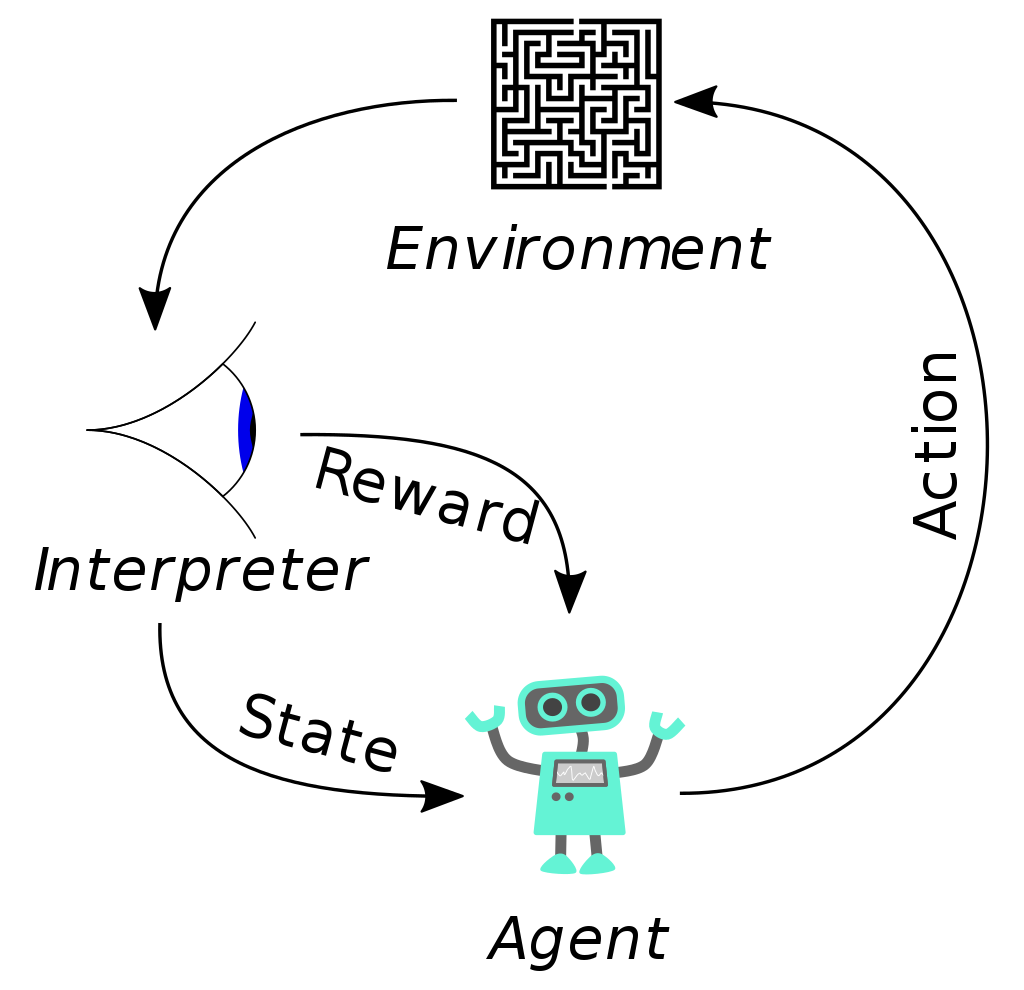
\includegraphics[scale=.1]{rl.png}
						\end{figure}
					\end{column}

					\begin{column}{0.5\textwidth}
					\begin{figure}
						\centering
						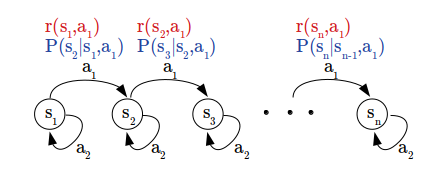
\includegraphics[scale=.4]{state_machine_1.png}
					\end{figure}
					\end{column}

				\end{columns}
				\item As well as with a mathematical formula: $v(s) = \textcolor{red}{r(s,a)}+ \gamma \sum_{j \in \mathcal{S}} \textcolor{blue} {P(s_j | s,a)} v(j) $
			\end{itemize}

	\end{itemize}
% \hyperlinkslidenext{\beamerbutton{next}}
\end{frame}
%=====================================%
%=====================================%

\begin{frame}
	\frametitle{Value Function}
	\begin{itemize}
		\item It is a measure of how good is it to be at state $s$
		\item We like $v(s)$ to be as large as possible
		\[
			v^*(s) = \max_{a} \{r(s,a) + \sum_{j \in \mathcal{S}} {P(s_j | s,a)} v(j)\}
		\]
		\item There are many ways to solve this equation, such as \textcolor{blue}{Value Iteration, Policy Iteration, Dynamic Programming}, etc.
		\item The problem can also be formulated as a \textcolor{green}{Linear Program}
	\end{itemize}
\end{frame}
%=====================================%
%=====================================%

\begin{frame}
	\frametitle{Value Function Optimization Using LP}
	\begin{itemize}
		\item We are looking for the maximum of vector $v(s)$, which is of the size of the action set $|\mathcal{A}|$
		\[
			\begin{matrix}
				\min v(s) \\
				s.t. \quad v(s) \geq r(s,a) + \gamma \sum_{j \in \mathcal{S}} {P(s_j | s,a)} v(j) \quad \forall a \in \mathcal{A}
			\end{matrix}	
		\]
		\item We can do the same thing for all states
		\[
			\begin{matrix}
				\min \sum_{j \in \mathcal{S}} \alpha(j)v(j) \\
				s.t. \quad v(s) \geq r(s,a) + \gamma \sum_{j \in \mathcal{S}} {P(s_j | s,a)} v(j) \quad \forall a \in \mathcal{A} \quad \forall s \in \mathcal{S}
			\end{matrix}	
		\]
		\item In vector form, with a bit of factorization and simplification
		\[
			\begin{matrix}
				\min \alpha\top v \\
				s.t. \quad \underbrace{(E - \gamma P)}_{A} v \geq r
			\end{matrix}	
		\]		
	\end{itemize}
\end{frame}
%=====================================%
%=====================================%

\begin{frame}
	\frametitle{Value Function Optimization Using LP}
	Example:
	\begin{columns}
	
		\begin{column}{0.5\textwidth}
			\begin{figure}
				\centering
				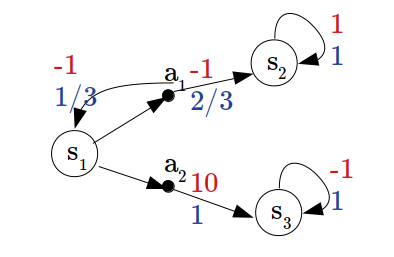
\includegraphics[scale=.4]{exmpl.png}
			\end{figure}
		\end{column}

		\begin{column}{0.5\textwidth}
		\begin{figure}
				\centering
				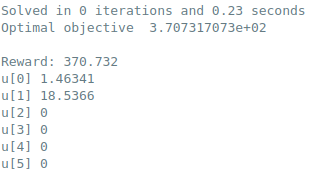
\includegraphics[scale=.6]{lp_gurobi.png}
			\end{figure}
		\end{column}

	\end{columns}


	
\end{frame}
%=====================================%
%=====================================%

\begin{frame}
	\frametitle{Robust MDPs}
	\begin{itemize}
		\item We learned that $v^*$ is
		\[
			\begin{matrix}
				\min \limits_v \alpha^\top v \\
				Av \geq r
			\end{matrix}	
		\]
		\item The dual of $v^*$ is
		\[
			\begin{matrix}
				\max \limits_u r^\top u \\
				A^\top u = \alpha \\
				u \geq 0
			\end{matrix}	
		\]
		\item In robust optimization, there are two agents. One is trying to maximize the objective function, and the other tries to minimize it
		\item In robust MDPs, nature plays the role of the second agent
		\[
			\begin{matrix}
				\max \limits_{r \in \mathcal{R}} \quad \max \limits_u r^\top u \\
				A^\top u = \alpha \\
				u \geq 0
			\end{matrix}	
		\]
	\end{itemize}
\end{frame}
%=====================================%
%=====================================%

\begin{frame}
	\frametitle{Robust MDPs}
	\begin{itemize}
		\item By strong duality we know
		\[
			\begin{matrix}
			
				\begin{matrix}
					\min \limits_{r \in \mathcal{R}} \quad \max \limits_u r^\top u  = \\
					A^\top u = \alpha \\
					u \geq 0
				\end{matrix}
				& 
				\begin{matrix}
					\max \limits_u \quad \min \limits_{r \in \mathcal{R}} r^\top u \\
					A^\top u = \alpha \\
					u \geq 0
				\end{matrix}
			\end{matrix}
		\]
		\item If the constraint over rewards are defined linearly ($Cr \leq d$)
		\[
			\begin{matrix}
				\max \limits_u & \min \limits_{r} r^\top u \\
				A^\top u = \alpha  & Cr \leq d\\
				u \geq 0
			\end{matrix}
		\]
		\item By writing the dual of the inner minimization and turn it into a maximization
		\[
			\begin{matrix}
				\max \limits_{u,t} d^\top t\\
				A^\top u = \alpha \\
				u \geq 0 \\
				C^\top t = u \\
				t \geq 0
			\end{matrix}
		\]
	\end{itemize}
\end{frame}
%=====================================%
%=====================================%

\begin{frame}
	\begin{center}
		\Huge Thank You!
	\end{center}
\end{frame}
%=====================================%

% %=====================================%

% \begin{frame}
% 	\frametitle{Background}
% 	\begin{itemize}

% 	\end{itemize}
% \end{frame}
% %=====================================%



%=====================================%

% \begin{frame}
% 	\begin{center}
% 		\Huge Thank You!
% 	\end{center}
% \end{frame}
%=====================================%

% \begin{frame}
	% \frametitle{Background}
% 	\begin{itemize}
% 		\item 
% 	\end{itemize}
% \end{frame}


\end{document}
